
\chapter{Bundles}

  The definition of a vector on a Manifold is non-trivial because a vector space structure might not exist globally on the manifold. A Manifold may still be equipped with a Vector space structure locally. Thus, tangent spaces are introduced pointwise. Combining these local structures will lead naturally to the definition of fiber bundles.

\section{Tangent Space $T_pM$}

  Let $M$ be an $n$-dimensional smooth manifold. A tangent vector at a point $p \in M$ is a linear map $v: C^\infty(M) \to \mathbb{R}$ satisfying the Leibniz rule \cite{FredericSchullerDifferentialstructurespivotalconcepttangentvectorspacesLec09FredericSchuller2015}:
 \[ v[fg] = v[f]g(p) + f(p)v[g] \]

  A tangent vector at a point $p \in M$ can be constructed as the directional derivatives of an equivalence class of curves through $p$\cite{NakaharaGeometrytopologyphysics2005}.

  Let $\gamma: [-\epsilon, \epsilon] \to M$ be a smooth curve in $M$ with $\gamma(0)=p$. Then $\phi \circ \gamma(t) = x(t) \in \mathbb{R}^n$ is called the coordinate representation of $\gamma$ induced by a chart $(U, \varphi)$.
Let $f \in C^\infty(M)$ be a smooth function on $M$. The directional derivative of $f$ along the curve $\gamma$ at $t=0$ is given by:
\begin{align*}
\left. \frac{d}{dt} (f \circ \gamma)(t) \right|_{t=0}
  &= \left. \frac{d}{dt} \left( f\circ \varphi^{-1}\circ\varphi\circ\gamma(t) \right) \right|_{t=0} \\[0.8em]
&= \left. \frac{\partial f}{\partial x^r} \frac{d x^r}{dt} \right|_{t=0} \\[0.8em]
&= \left. \frac{d x^r}{dt} \right|_{t=0} \left. \frac{\partial f}{\partial x^r} \right|_p
\end{align*}

The definition of a tangent vector is now obtained by introducing an equivalence relation on curves. Two curves $\gamma_1$ and $\gamma_2$ are called equivalent at $\gamma_1(0)=\gamma_2(0)=p$ if their derivatives at $t=0$ are equal:
\[
\left. \frac{d x_1^r}{dt} \right|_{t=0}
= \left. \frac{d x_2^r}{dt} \right|_{t=0}
= v^r
\]
A tangent vector is identified with the differential operator given the equivalence class of curves. Once a chart $(U, \varphi)$ is chosen, with local coordinates $(x^1, \dots, x^n)$, a tangent vector is represented as a linear combination of partial derivatives with real coefficients.
\[
v = v^r \left. \frac{\partial}{\partial x^r} \right|_p
\]
The tangent space at a point $p \in M$ is then defined as the set of all tangent vectors at $p$ and is denoted by $T_pM$.
\[
\left\{ \left. \frac{\partial}{\partial x^1} \right|_p, \dots, \left. \frac{\partial}{\partial x^n} \right|_p \right\} \quad \text{form a basis of } T_pM
\]



\section{The Tangent Bundle as a Fiber Bundle}

To introduce the concept of fiber bundles, a detailed examination of a specific example, the tangent bundle, serves as an effective foundation.
The tangent bundle of a smooth \( n \)-dimensional manifold \( M \) is constructed by taking the disjoint union of all tangent spaces \( T_pM \). This construction can be represented as:
\[
TM := \bigsqcup_{p \in M} T_pM = \bigcup_{p \in M} \{p\} \times T_pM
\]
Here, \( T_pM \) denotes the tangent space at a point \( p \in M \). The tangent space \( T_pM \) is a vector space that consists of all tangent vectors at the point \( p \). It should be noted that this notation emphasizes the pointwise nature of the disjoint union, where each tangent space is associated with a specific point on the manifold. Since each tangent space is a different object, a certain tangent vector in a tangent space can only belong to that specific tangent space. Therefore all the information is already in the vector itself and the direct product notation \( \{p\} \times T_pM \) is only used to clarify \cite{FredericSchullerTopologicalmanifoldsmanifoldbundlesLec06FredericSchuller2015}.

Each element of the tangent bundle \( TM \) can be expressed as a pair \( (p, v) \), where \( p \) is a point on the manifold \( M \), and \( v \) is a tangent vector belonging to the tangent space \( T_pM \) at that point. 
A natural projection map is defined as follows:
\[
\pi: TM \to M, \quad (p, v) \mapsto p
\]
This projection, \( \pi \), serves to "forget" the tangent vector \( v \) associated with each point, effectively collapsing all the tangent vectors at \( p \) to the single point \( p \) in the base manifold \cite{NakaharaGeometrytopologyphysics2005}.

The fiber over a point \( p \) is denoted as \( \pi^{-1}(p) = T_pM \). This represents all the tangent vectors at the point \( p \). Since \( T_pM \) is isomorphic to \( \mathbb{R}^n \) as a vector space, it is referred to as the model fiber, denoted \( F = \mathbb{R}^n \) \cite{NakaharaGeometrytopologyphysics2005}.
Since the fiber of the tangent bundle is a vector space, the tangent bundle is also referred to as a \textbf{vector bundle}.

Consider a coordinate chart \( (U, \varphi) \) on \( M \). The chart \( \varphi \) provides a mapping from an open set \( U \subseteq M \) to an open subset of \( \mathbb{R}^n \). A diffeomorphism on the preimage \( \pi^{-1}(U) \subset TM \) can then be defined as:
\[
\Psi: \pi^{-1}(U) \to \mathbb{R}^{2n}, \quad (p, v) \mapsto \left(x^1(p), \dots, x^n(p), v^1, \dots, v^n \right)
\]
where the coordinates \( x^i(p) \) represent the local coordinates of the point \( p \) in \( U \), and \( v = v^i \left. \frac{\partial}{\partial x^i} \right|_p \) describes the tangent vector in terms of its components in the chosen coordinate system \cite{NakaharaGeometrytopologyphysics2005}.
This establishes a local trivialization of the tangent bundle, expressed as:
\[
TM|_U \cong U \times \mathbb{R}^n
\]

In summary, the construction of the tangent bundle yields a fiber bundle characterized by the following essential components:
\begin{itemize}
  \item \textbf{Total space:} \( TM = \bigsqcup_{p \in M} T_pM \), encapsulating all tangent spaces.
  \item \textbf{Base space:} \( M \), a manifold to which additional structure is added.
  \item \textbf{Projection:} \( \pi: TM \to M \), mapping each tangent vector to its associated point on the manifold.
  \item \textbf{Model fiber:} \( F = \mathbb{R}^n \), serving as the standard fiber structure over each point.
  \item \textbf{Local trivialization:} \( TM|_U \cong U \times \mathbb{R}^n \), ensuring that the tangent bundle locally resembles a product structure.
\end{itemize}

 Similar to the way a manifold is commonly perceived as a space that locally resembles \( \mathbb{R}^n \), a fiber bundle may be conceptualized as a space that locally resembles the Cartesian product of the base space with a typical fiber structure. 


\section{Definition of a Fiber Bundle}

The formal definition of a fiber bundle reads as follows\cite{FredericSchullerTopologicalmanifoldsmanifoldbundlesLec06FredericSchuller2015, DudekEhreshmanntheoryconnectionprincipalbundlecompendiumphysicists2018}.
A fiber bundle is a quadruple $(E, B, \pi, F)$ where:
\begin{itemize}
  \item $E$ is the total space
  \item $B$ is the base space
  \item $\pi: E \to B$ is a surjective map called the projection
  \item $F$ is the typical fiber
\end{itemize}

There exists an open cover $\{U_\alpha\}$ of $B$ such that for each $\alpha$, there is a diffeomorphism
\[
\varphi_\alpha: \pi^{-1}(U_\alpha) \to U_\alpha \times F
\]
such that the following diagram commutes:


\begin{center}
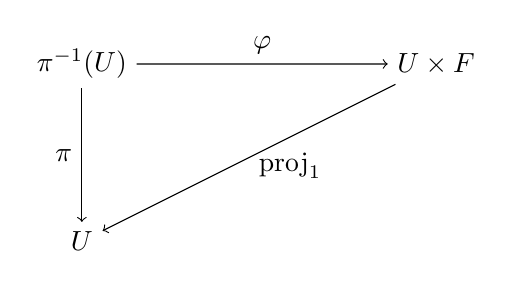
\begin{tikzpicture}[scale=1.5, every node/.style={font=\normalsize}]
  \node (A) at (0,1.5) {$\pi^{-1}(U)$};
  \node (B) at (3,1.5) {$U \times F$};
  \node (C) at (0,0) {$U$};

  \draw[->] (A) -- (B) node[midway, above] {$\varphi$};
  \draw[->] (A) -- (C) node[midway, left] {$\pi$};
  \draw[->] (B) -- (C) node[midway, right, yshift=-3pt] {$\mathrm{proj}_1$};
\end{tikzpicture}
\end{center}


where $\text{proj}_1: A \times B \to A$ is the first projection. $(U_\alpha, \varphi_\alpha)$ are called \emph{local trivialization}. The fiber over a point $b \in B$ is:
\[
F_b := \pi^{-1}(\{b\}) \cong F
\]

Often the notations $E \xrightarrow{\pi} B$ or $\pi : E \to B$ are used to denote a fiber bundle.


\subsection{The Structure Group of a Fiber Bundle}

Above a fiber bundle was defined as a quadruple \((E, B, \pi, F)\) equipped with local trivializations. These local trivializations are established as diffeomorphisms on an open cover $\{U_\alpha\}$ of the base space \(B\). The definition does not impose the requirement that \(U_\alpha \cap U_\beta = \emptyset\). For a point \(p \in U_\alpha \cap U_\beta\), multiple local trivializations \(\varphi_\alpha(p, f) = \varphi_{\alpha,p}(f)\) and \(\varphi_\beta(p, f) = \varphi_{\beta,p}(f)\) may be present, defined on \(U_\alpha\) and \(U_\beta\), respectively.

The \textbf{structure group} \(G\) of a fiber bundle is defined as the Lie group of diffeomorphisms relating these local trivializations. The corresponding transition function is given by\cite{NakaharaGeometrytopologyphysics2005}:

\[
t_{\alpha\beta}(p) \equiv \varphi_{\alpha,p}^{-1} \circ \varphi_{\beta,p} : F \to F
\]

This establishes a smooth map \(t_{\alpha\beta}: U_\alpha \cap U_\beta \to G\) that satisfies the following properties:

\begin{align*}
  t_{\alpha \alpha}(p) &= \mathrm{id}_F && \forall\, p \in U_\alpha \\
  t_{\alpha\beta}(p) &= t_{\beta\alpha}(p)^{-1} && \forall\, p \in U_\alpha \cap U_\beta \\
  t_{\alpha\beta}(p) \circ t_{\beta\gamma}(p) &= t_{\alpha\gamma}(p) && \forall\, p \in U_\alpha \cap U_\beta \cap U_\gamma
\end{align*}

In the case of the tangent bundle, the structure group corresponds to the general linear group \(\mathrm{GL}(n, \mathbb{R})\), which consists of all invertible \(n \times n\) matrices. 
A fiber bundle where all transition maps can be chosen to be the identity map is termed a \textbf{trivial bundle}. In this scenario, the total space \(E\) is diffeomorphic to the product space \(B \times F\). 

Generally, a fiber bundle does not possess a unique trivialization. Let \(\{\varphi_\alpha\}\) and \(\{\tilde{\varphi}_\alpha\}\) denote two local trivializations over the same open covering that describe the same fiber bundle. These trivializations are related by maps \(g_\alpha(p) : F \to F \quad \forall\, p \in B\), where each \(g_\alpha(p)\) is a homeomorphism within the structure group \(G\). The transition function between the two local trivializations is then given by:

\[
g_\alpha(p) \equiv \varphi_{\alpha,p}^{-1} \circ \tilde{\varphi}_{\alpha,p}
\]

Considering the tangent bundle as an illustrative example\cite{NakaharaGeometrytopologyphysics2005}, let \(U_i\) and \(U_j\) represent overlapping charts with \(p \in U_i \cap U_j\). Utilizing the basis \(\left\{ \left. \frac{\partial}{\partial x^i} \right|_p \right\}\) and \(\left\{ \left. \frac{\partial}{\partial y^j} \right|_p \right\}\), a vector \(v \in T_pM\) can be expressed in both bases as:

\[
v = v^{\mu} \frac{\partial}{\partial x^{\mu}} = \tilde{v}^{\mu} \frac{\partial}{\partial y^{\mu}}
\]

The transition function \(t^\nu_{\,\,\mu}\) is thus defined as:

\[
\tilde{v}^\nu = \left.\frac{\partial y^\nu}{\partial x^\mu}\right|_p v^\mu = t^\nu_{\,\,\mu} v^\mu
\]

\subsection{Sections}

An important definition in the context of fiber bundles is that of a section or cross-section. This concept enables the selection of an element from each fiber over each point in a continuous manner, facilitating the introduction of ideas such as vector fields over spacetime\cite{NakaharaGeometrytopologyphysics2005}.

A \textbf{section} of a fiber bundle \(\pi : E \to B\) is defined as a continuous map \(s: B \to E\) such that

\[
\pi \circ s = \mathrm{id}_B.
\]

This condition ensures that exactly one point is chosen from each fiber continuously. 
The set of all (smooth) sections is denoted by:
\[
\Gamma(E) := \left\{ s: M \to E \mid \pi \circ s = \mathrm{id}_{M} \right\}.
\]
It is also possible to define a section locally on an open set \(U \subset B\) as a map \(s: U \to E\) such that \(\pi \circ s = \mathrm{id}_U\). In this case, the section is called a \textbf{local section}.
For example, a vector field over a manifold $M$ can therefore be understood as a section of the tangent bundle \(TM\) over \(M\).

\section{The cotangent bundle and differential forms}

\subsection{The Cotangent Bundle}
In this section the fundamental concepts of the cotangent bundle are introduced, which is essential for the definition of differential forms and the exterior derivative. The cotangent space at a point $p$ on a manifold $M$ is defined as the dual space of the tangent space at that point. Formally, the cotangent space at a point $p \in M$ is the set of all linear maps from the tangent space at that point to the real numbers\cite{NakaharaGeometrytopologyphysics2005}.
\[
T_p^*M := \text{Hom}_\mathbb{R}(T_p M, \mathbb{R})
\]
A covector \(\omega \in T_p^*M\) is such a linear function:
\[
\omega: T_p M \to \mathbb{R}
\]
As an example, consider a function \(f \in C^\infty(M)\) and some tangent vector $v \in T_pM$. Then $v[f] \in \mathbb{R}$ by definition. The differential of \(f\) at a point \(p\) is a covector $df_p$ and therefore $df_p[v]\in \mathbb{R}$ is simply defined as $df_p[v] = v[f]$.
Given a coordinate basis \(\left\{ \left. \frac{\partial}{\partial x^i} \right|_p \right\}\)  of \(T_p M\) the dual basis is:
\[
\left\{ \left. dx^i \right|_p \right\}
\]
satisfying the relation:
\[
dx^i\left( \left. \frac{\partial}{\partial x^j} \right|_p \right) = \delta^i_j
\]
The example from before can thus be expressed as:
\[
df_p = \frac{\partial f}{\partial x^i} dx^i \quad \text{and} \quad df_p[v] = v^i \left. \frac{\partial f}{\partial x^i} \right|_p
\]
Analogous to the tangent bundle, the cotangent bundle is defined as the disjoint union of all cotangent spaces at each point in the manifold:
\[
T^*M := \bigsqcup_{p \in M} T_p^* M
\]
This structure constitutes a vector bundle over \(M\). A section of the cotangent bundle can be defined as:
\[
\omega \in \Gamma(T^* M)
\]
This section assigns to each \(p \in M\) a covector \(\omega_p \in T_p^*M\) smoothly. Such a section is referred to as a \textbf{1-form}. In a coordinate representation, a 1-form can be expressed as:
\[
\omega = \sum_{i=1}^n \omega_i(x) \, dx^i
\quad \text{with} \quad \omega_i \in C^\infty(M)
\]

\subsection{Tensor Fields and the Metric Tensor}

Utilizing the fact that the fibers of the cotangent bundle are vector spaces, tensor products of bundles can be defined. For instance:
\[
T^*M \otimes T^*M := \bigsqcup_{p \in M} T_p^*M \otimes T_p^*M
\]
This forms a bundle whose fibers consist of maps form $TM \otimes TM$ to $\mathbb{R}$. Sections of this bundle are referred to as \((0,2)\)-tensor fields. A prominent example of such fields is the metric tensor. The Minkowski metric is defined as:
\[
\eta \in \Gamma(T^*M \otimes T^*M)
\]
In local coordinates, the Minkowski metric can be expressed as:
\[
\eta = \eta_{\mu\nu} \, dx^\mu \otimes dx^\nu
\quad \text{with} \quad \eta_{\mu\nu} = \text{diag}(1, -1, -1, -1)
\]
In general, a tensor field of type $(i,j)$ is a section of the bundle \cite{NakaharaGeometrytopologyphysics2005}:
\[ \otimes^iT^*M \otimes^jTM \]


\subsection{Differential Forms and the Exterior Derivative}
A \textbf{k-form} or \textbf{differential form} of order k is a totally antisymmetric $(k,0)$ tensor. To define a k-form, it is necessary to take the \textbf{wedge product} of 1-forms, which is defined by taking the totally antisymmetrized tensor product of 1-forms. This means that all permutations of the tensor product are considered, with even permutations contributing positively and odd permutations contributing negatively. Consider the cotangent space $T_p^*M$ of a manifold $M$ at a point $p$ with basis $\{dx^\mu\}$. The wedge product of two 1-forms \(dx^\mu\) and \(dx^\nu\) thus reads:
\[
dx^\mu \wedge dx^\nu = dx^\mu \otimes dx^\nu - dx^\nu \otimes dx^\mu
\]
Higher order forms can be constructed analogously. By taking the cotangent bundle \(T^*M\) and considering the antisymmetrized tensor product, we can define fields of differential forms of order \(r\) as:
\[\Omega^r(M) \equiv \Gamma(\wedge^r (T^*M))\]

The \textbf{exterior derivative} is then defined as a map \cite{NakaharaGeometrytopologyphysics2005}:
\begin{align*}
  d: \Omega^r(B) &\to \Omega^{r+1}(B) \\
  \omega &\mapsto d\omega = \frac{1}{r!}\left( \frac{\partial}{ \partial x^\nu} \omega_{\mu_1 \dots \mu_r} \right) dx^\nu \wedge dx^{\mu_1} \wedge \dots \wedge dx^{\mu_r}
\end{align*}

In the following, two relations will be shown that will be used in later proofs \cite{NakaharaGeometrytopologyphysics2005}. First consider the action of the exterior derivative on a 1-form $\omega=\omega_\mu dx^\mu \in \Omega^1(M)$ on two tangent vector fields $v=v^\mu\frac{\partial}{\partial x^\mu}$ and $w=w^\nu\frac{\partial}{\partial x^\nu}$:
\begin{align*}
  d\omega(V, W) 
  &= \left( \frac{\partial \omega_\mu}{\partial x^\nu} \, dx^\nu \wedge dx^\mu \right)(V, W) \\
  &= \frac{\partial \omega_\mu}{\partial x^\nu} 
  \left( dx^\nu(V) \, dx^\mu(W) - dx^\nu(W) \, dx^\mu(V) \right) \\
  &= \frac{\partial \omega_\mu}{\partial x^\nu} 
  \left( V^\nu W^\mu - W^\nu V^\mu \right) \\
  &= V^\nu \frac{\partial}{\partial x^\nu} \left( \omega_\mu W^\mu \right)
  - W^\nu \frac{\partial}{\partial x^\nu} \left( \omega_\mu V^\mu \right)
  - \omega_\mu \left( V^\nu \frac{\partial W^\mu}{\partial x^\nu} - W^\nu \frac{\partial V^\mu}{\partial x^\nu} \right) \\
  &= V[\omega(W)] - W[\omega(V)] - \omega([V, W])
\end{align*}
This gives a coordinate free expression for the action of the exterior derivative of a 1-form. Furthermore, it can easily be shown that the exterior derivative of a exterior derivative is zero, by using the fact that the product of a symmetric and an antisymmetric tensor is zero. By definition the following is obtained:
\[ d^2\omega = \frac{1}{r!}\left( \frac{\partial^2}{ \partial x^\alpha x^\beta} \omega_{\mu_1 \dots \mu_r} \right) dx^\alpha \wedge dx^\beta \wedge dx^{\mu_1} \wedge \dots \wedge dx^{\mu_r} \]
From this it follows instantly that $d^2=0$ since $\frac{\partial^2}{ \partial x^\alpha x^\beta}$ is symmetric and the wedge product is antisymmetric.


